\documentclass{article}
\usepackage[utf8]{inputenc}
\usepackage{algpseudocode}
\usepackage{graphicx}
\graphicspath{ {./img/} }

% for headers
\usepackage{fancyhdr}
\pagestyle{fancy}

% for automatas
\usepackage{tikz}
\usetikzlibrary{automata,positioning}

% for \mod and \text in math mode
\usepackage{amsmath}

% for \mathbb{N}
\usepackage{amsfonts}

% metadata
\title{Problème du plus court vecteur dans les réseaux
\\ Projet de session du cours INF889B}
\author{Félix Larose-Gervais}
\date{Décembre 2023}

% defining variables
\setlength{\headheight}{24pt}
\makeatletter
\let\theTitle\@title{}
\let\theAuthor\@author{}
\let\theDate\@date{}
\makeatother

% headers
\lhead{\theTitle}
\rhead{\theAuthor}

% start
\begin{document}

% first page
\begin{titlepage}
\maketitle
\thispagestyle{empty}
\end{titlepage}

\tableofcontents

\newpage

\section{Introduction}

Cet article porte sur le problème du plus cours vecteur dans les réseaux (souvent nommé SVP, de l'anglais Shortest Vector Problem), sujet de mon projet de session lors du cours INF889B (Algorithmes d'optimisation combinatoire). On y explore la manière d'énumérer l'espace de solutions, puis comment accélérer la recherche via diverses techniques d'optimisation.

\subsection{Motivation}

Le sujet est d'intérêt puisque sa difficulté supposée forme la base de plusieurs crypto-systèmes émergents. En effet, la sécurité de plusieurs crypto-systèmes modernes tels que RSA et Diffie-Hellman reposent sur l'hypothèse que la factorisation entière et le logarithme discret sont des problèmes difficiles. Cependant, l'algorithme quantique de Shor vient mettre en péril cette supposition. Or, il est cru que les problèmes sur les réseaux euclidiens comme le SVP sont difficiles même pour un ordinateur quantique. Les systèmes basés sur ce problème sont aussi les seuls connus à ce jours pour être totalement homomorphes, une propriété désirable pour permettre la délégation de calcul respectant la vie privée.

\subsection{Définitions}

\subsubsection{Réseaux euclidiens}

Un réseau d'un espace vectoriel euclidien est un sous-groupe discret de l'espace.

Soient $n \in \mathbb{N}$ et $B \in GL_n(\mathbb{R})$ appelée une base, on définit le réseau $\mathcal{L}$ ainsi:

\[
    \mathcal{L}(B) = \{ Bx \mid x \in \mathbb{Z}^n \} \subset \mathbb{R}^n
\]

C'est-à-dire l'ensemble des points atteignables par une combinaison linéaire entière des colonnes de la base. On note que le réseau dépend de la base, en effet, plusieurs bases peuvent engendrer le même réseau.

\begin{figure}[h]
    \caption{Une base de $\mathbb{Z}^2$}
    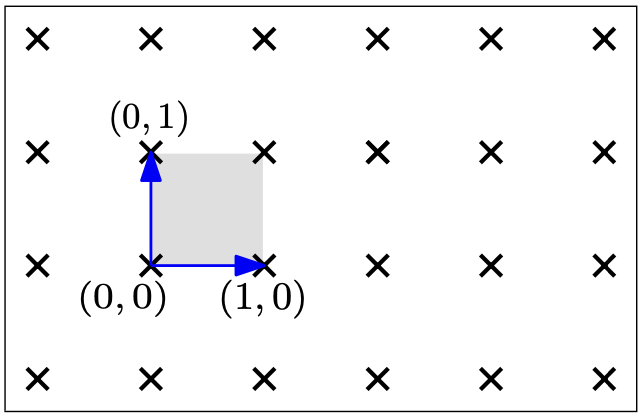
\includegraphics[width=8cm]{lattice.png}
    \centering
\end{figure}

\subsubsection{Problème du vecteur le plus court}

Étant donné un réseau $\mathcal{L}$, notons la longueur de son plus petit vecteur non nul:

\[
    \lambda(\mathcal{L}) = \min_{v \in \mathcal{L} \setminus \{0\}} { \lVert v \rVert }
\]

où $\lVert v \rVert$ dénote ici la norme euclidienne, avec $v = (v_1, \dots, v_n)$:

\[
    \lVert v \rVert = \sqrt{v_1^2 + \cdots + v_n^2}
\]

Le problème consiste à trouver un tel $v$ non nul minimisant la norme étant donné un réseau de base $B$. Ce problème est connu pour être NP-Difficile.

\begin{figure}[h]
    \caption{Le vecteur le plus court d'un réseau}
    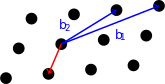
\includegraphics{SVP.png}
    \centering
\end{figure}

\subsection{Méthode naïve}

A priori, il suffit d'énumérer les points du réseau, et choisir celui minimisant la norme. Cependant, il en existe un nombre infini. Pour pouvoir compléter l'énumération, il faut borner les coefficients de la combinaison linéaire entière, tout en garantissant qu'un vecteur de longueur $\lambda$ se trouve dans l'espace de recherche.

Une telle borne est présentée par U. Dieter dans son article `How to calculate shortest vectors in a lattice`~\cite{svp}.

Il suffit de calculer la base du réseau dual de $\mathcal{L}$ c'est-à-dire \[D = B^{-T}\] 

Puis, étant donné une borne supérieure $w$ sur $\lambda$ (prenons la norme du plus petit vecteur de la base $B$), on peut borner nos coefficients entiers comme suit
\[
    |x_i| \leq \lVert d_i \rVert w
\]

avec $x_i \in \mathbb{Z}$ les coefficients entiers à énumérer et $d_i \in \mathbb{R}^n$ les colonnes de $D$. Pour chaque dimension, on a donc $2 \lVert d_i \rVert w + 1$ entiers à énumérer, c'est-à-dire un nombre exponentiel en $n$ de points à énumérer en tout.

\begin{align*}
    \prod_{i=1}^{n}{2 \lVert d_i \rVert w + 1}
    = 2^n w^n n \prod_{i=1}^{n}{\lVert d_i \rVert } + \cdots + 1
    \in O(2^n)
\end{align*}

\section{Optimisation combinatoire}

On explore dans cette sections plusieurs améliorations possibles à l'algorithme naïf présenté plus haut. Bien que la difficulté du problème croisse fondamentalement de manière exponentielle par rapport à la dimension du réseau, il est possible d'appliquer des techniques d'optimisation accélérant drastiquement la recherche du plus court vecteur.

\subsection{Symmétrie}

Tout d'abord, notons que, comme $\mathcal{L}$ est un groupe additif, chaque vecteur $v \in \mathcal{L}$ possède un inverse noté $-v \in \mathcal{L}$. Et puisque $\forall r \in \mathbb{R}: r^2 = {(-r)}^2$, on constate 
\[ \lVert v \rVert = \lVert -v \rVert \]

Sachant cela, il est inutile d'énumérer tous les points de notre espace borné. Étant donné un vecteur de coefficients $x \in \mathbb{Z}^n$ générant un point $v = Bx \in \mathcal{L}$, on a pas besoin de générer $-v = B(-x) \in \mathcal{L}$.

Pour ce faire, on observe d'abord qu'un point passant par l'origine coupe la droite réelle en deux, puis qu'une ligne (n'importe laquelle) passant par l'origine coupe le plan en deux, et que n'importe quel plan passant par l'origine coupe l'espace en deux. Plus généralement, un hyperplan de dimension $n-1$ passant par l'origine coupe l'espace de dimension $n$ en deux.

Cela nous permet de prendre n'importe quel axe de l'espace et ne considérer que les points d'un de ses côtés lors de l'énumération. On peut arbitrairement choisir de ne considérer que les valeurs positives de la première coordonnée du vecteur de coefficients.

\begin{figure}[h]
    \caption{Deux vecteurs opposés ont la même norme}
    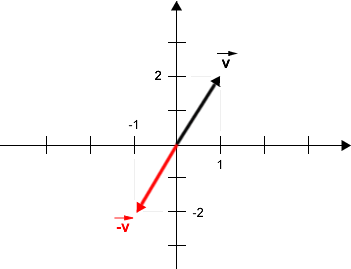
\includegraphics[width=8cm]{symm.png}
    \centering
\end{figure}

\subsection{Séparation et évaluation}

Cette méthode, connue en anglais sous le nom de ``Branch and bound'' est une technique répandue en optimisation combinatoire visant à réduire successivement l'espace de recherche pendant l'énumération. On peut voir l'espace de recherche comme un arbre de profondeur $n$ ou chaque niveau correspond à un choix d'une coordonée du vecteur de coefficients générant les points de $\mathcal{L}$. La méthode d'énumération présentée consiste à parcourir cet arbre, considérant un point généré par le chemin de la racine vers chaque feuille en cherchant celui dont la norme serait minimale. Couper des branches de cet arbre peut réduire drastiquement le nombre de points à considérer.

Pour ce faire, rappelons que les bornes des coordonnées sur les vecteurs de coefficients à énumérer sont obtenues à partir d'une borne supérieure $w$ sur $\lambda$. Lors de l'énumération, chaque fois que l'on trouve un nouveau vecteur plus court que le précédent, on peut mettre à jour cette borne supérieure, et du même coup les bornes des coefficients.

Afin d'éviter de couper une branche déjà explorée, il peut être intéressant de modifier l'ordre d'énumération naturel sur les entiers (de la borne inférieure vers la borne supérieure) et de plutôt partir du centre (zéro) et évoluer autour en spirale vers les bornes. Ainsi les $x_i$ prennent des valeurs successives $0, 1, -1, 2, -2, \dots$ et on ne découvre jamais a posteriori qu'un point déjà énuméré ne pouvait pas être optimal.

\subsection{Traitement par lots}

La génération d'un point du réseau consiste à multiplier une matrice carrée $B \in GL_n(\mathbb{R})$ (la base du réseau) par un vecteur de coefficients $x \in \mathbb{Z}^n$. Cette opération est effectuée un nombre exponentiel en $n$ de fois et demande donc à être accélérée autant que possible. Regrouper $n$ tels vecteurs en une matrice carrée $X$ et calculer le produit matriciel $BX$ nous donne une nouvelle matrice carrée dont les colonnes sont $n$ points du réseau. Un tel traitement semble à priori équivalent en terme de calcul, mais l'utlisation d'un algorithme de multiplication de matrice efficace comme celui de Strassen pourrait être un accélérant.

Cependant, il a été empiriquement observé sur des petites instances du problème ($n < 100$) que cette technique ralentissait en fait la recherche, probablement dû aux allocations supplémentaires, défauts de cache encourus et multiples opérations élémentaires additionnelles. Il n'est pas à exclure que cette méthode pourrait tout de même être efficace sur de beaucoup plus larges instances du problème ($n > 1000$), moyennant une implémentation adéquate minimisant les allocations.

\newpage

\subsection{Approximation}

Le problème de recherche SVP admet aussi une variante d'approximation $\gamma$-SVP cherchant à trouver un vecteur $v$ tel que $\lVert v \rVert \leq \gamma \lambda$. Une telle approximation $v$ peut ensuite être utilisée pour calculer des bornes de recherche pour la version exacte du problème. LLL est un algorithme s'exécutant en temps polynomial en $n$ trouvant une solution à $2^{O(n)}$-SVP. Il permet donc de rapidement trouver une approximation qui réduit potentiellement beaucoup l'espace de recherche.

\section{Algorithme LLL}

L'algorithme LLL, dû à Lenstra, Lenstra et Lovász\cite{lll}, prend en entrée la base d'un réseau, et produit une nouvelle base équivalente (c'est-à-dire engendrant le même réseau) dite LLL réduite. Cette nouvelle base a la propriété que son plus petit vecteur est une $2^{O(n)}$-approximation de $\lambda$.

\subsection{Orthogonalisation de Gram-Schmidt}

Soient $n \in \mathbb{N}$, $B = \{ b_1, \dots, b_n\} \in GL_n(\mathbb{R})$, notons $B^* = \{ b_1^*, \dots, b_n^* \} \in GL_n(\mathbb{R})$ le résultat de l'orthogonalisation de $B$ par le procédé de Gram-Schmidt. Pour l'obtenir, on pose $b_1^* = b_1$, puis pour les $k$ de 2 à $n$:

\[ b_k^* = b_k - \sum_{j=1}^{k-1}{\mu_{j, k}b_j}\]

où $\mu_{j, k} = \frac{\langle b_k, b_j \rangle}{\langle b_j, b_j \rangle }$ et $\langle \cdot, \cdot \rangle$ dénote le produit scalaire

\subsection{Réduction de base}

Une base $B = \{ b_1, \dots, b_n\} \in GL_n(\mathbb{R})$ est dite $\delta$-LLL réduite si, pour $\delta \in (0.25, 1)$
\[ \forall j < i : |\mu_{i, j}| \leq 0.5 \]
\[ \forall k \in [2, n] : \delta \lVert b_{k-1}^*\rVert^2 \leq \lVert b_k^* \rVert^2 + \mu_{k,k-1}^2 \lVert b_{k-1}^* \rVert^2 \]

Une propriété importante d'une base $\delta$-LLL réduite est que son premier vecteur est une approximation du vecteur le plus court:
\[ \lVert b_1 \rVert \leq \left( \frac{2}{\sqrt{4\delta-1}} \right) ^{n-1} \lambda \]

\newpage

\subsection{Procédure principale}

L'algorithme réduit la base donnée par des approximation entières de ses coefficients de Gram-Schmidt successives jusqu'à ce que la condition de Lovász soit satisfaite.

\begin{algorithmic}
    \State{\textbf{Input} Basis $b_1, \dots, b_n$}
    \Loop{}
        \State{Calcule $\tilde{b}_1, \dots, \tilde{b}_n$ par Gram-Schmidt}
        \State{// Étape de réduction}
        \For{$i = 2$ to $n$} 
            \For{$j = i - 1$ to $1$}
                \State{$b_i \gets b_i - \lfloor \mu_{i, j} \rceil b_j$}
            \EndFor{}
        \EndFor{}
        \State{// Condition de Lovász}
        \If{$\exists i : \lVert \tilde{b}_{i+1} \rVert < \sqrt{\delta - \mu_{i+1,i}^2} \lVert \tilde{b}_i \rVert $}
            \State{Swap $b_i$ et $b_{i+1}$}
        \Else{}
            \State{\Return{$b_1, \dots, b_n$}}
        \EndIf{}
    \EndLoop{}
\end{algorithmic}

\subsection{Exemple}

Soit $B \in GL_3(\mathbb{Z})$ la base d'un réseau euclidien
\[ 
    B = \begin{bmatrix} 
        1 & -1 & 3 \\ 
        1 & 0 & 5 \\ 
        1 & 2 & 6 
    \end{bmatrix} 
\]
On peut y appliquer l'algorithme LLL afin de produire la base réduite
\[
    \tilde{B} = \begin{bmatrix}
        0 & 1 & -1 \\
        1 & 0 & 0 \\
        0 & 1 & 2
    \end{bmatrix}
\]

On constate aussi que la première colonne de $\tilde{B}$ est directement le vecteur le plus court de l'espace engendré par $B$ et $\tilde{B}$. Ce n'est pas le cas en général mais la réduction LLL donne en pratique une bonne approximation du vecteur le plus court et accélère donc grandement la recherche.

\newpage

\section{Benchmark}

Lors du projet, une implémentation\footnote{https://github.com/filedesless/classes/tree/main/INF889B/svp} rust du problème avec les diverses optimisations présentées a été réalisée. Ensuite, différentes bases on été générées via SAGEMATH afin de comparer l'efficacité des optimisations.

\subsection{Instance aléatoire}

L'instance aléatoire correspond à une instance simple du problème; c'est-à-dire une matrice 10$\times$10 quelconque de déterminant 11.

\begin{center}
    \begin{tabular}{ |c|c| }
        \hline
        Optimisation & Temps moyen \\
        \hline
        Naive & 1794 ms \\
        Symmétrie & 1076 ms \\
        Coupure & 620 ms \\
        LLL & 13 ms \\
        \hline
        Combinées & 8 ms \\
        \hline
    \end{tabular}
\end{center}

\subsection{Instance difficile}

L'instance difficile est aussi une matrice 10$\times$10, mais de déterminant 28551. Ces matrices sont d'une classe montrée asymptotiquement difficile par M. Atjai\cite{hard} et sont plus pertinentes pour un usage en cryptographie.

\begin{center}
    \begin{tabular}{ |c|c| }
        \hline
        Optimisation & Temps moyen \\
        \hline
        Naive & ~16 m \\
        Symmétrie & ~8 m \\
        Coupure & 3.2 s \\
        LLL & 35 ms \\
        \hline
        Combinées & 21 ms \\
        \hline
    \end{tabular}
\end{center}

\section{Conclusion}

Dans cet article, on étudie le problème du plus court vecteur dans les réseaux euclidiens. Ce problème présente un intérêt comme base à la cryptographie post-quantique et au chiffrement homomorphe. On aborde plusieurs optimisations accélérant la recherche de solution et constate que la plus efficace passe par l'approximation (grâce à l'algorithme de réduction de base LLL) afin de rapidement réduire grandement l'espace de recherche.

\newpage

\bibliographystyle{unsrt}
\bibliography{refs} % Entries are in the refs.bib file




\end{document}